\chapter{Méthodes et outils d'études de la téhorie de l'évolution : expériences, modèles et Robotique}

\section{Méthodes et outils traditionnel}
\subsection{L'analogie Sélection artificielle \& Selection Naturelle}\label{sec:cmpdr:sa}

\begin{quote}
	Il est donc de la plus haute importance d'élucider quels sont les moyens de modification et de coadaptation. Tout d'abord, il m'a semblé probable que l'étude attentive des animaux domestiques et des plantes cultivées devait offrir le meilleur champ de recherches pour expliquer cet obscur problème. Je n'ai pas été désappointé ; j'ai bientôt reconnu, en effet, que nos connaissances, quelque imparfaites qu'elles soient, sur les variations à l'état domestique, nous fournissent toujours l'explication la plus simple et la moins sujette à erreur. Qu'il me soit donc permis d'ajouter que, dans ma conviction, ces études ont la plus grande importance et qu'elles sont ordinairement beaucoup trop négligées par les naturalistes.\footnote{\citet[Introduction]{darwin1859originspeciesbymeansnaturalselectionorpreservationfavouredracesstrugglelife}	D'après l'édition de 1896 (- SCHLEICHER FRERES, EDITEURS -).Traduit sur l'édition anglaise définitive par ED. BARBIER.
}
\end{quote}

C'est ainsi que dès l'introduction de son livre, Darwin place l'analogie entre sélection naturelle et sélection artificielle comme centrale dans son argument. Et en effet, tout au long de l'Origine des espèce Darwin n'aura de cesse de s'y référer, multi-pliant les exemple les chiens, les pigesons, les chevaux, presque toutes les espèces domestiques y passent. 

L'utilisation et la place de cette analogie a été beaucoup débattue par les philosophe de la fin du XXe siècles. Lui à-t-elle permis de compnre la selection naturelle, ou bien lui a-t-elle simplement permis de convaincre et d'illustre? 
Quelques soit la réponse à ces question il n'en demeure pas moins qu'elle à eu une place importangte 

Une des méthodes les plus utilisé en science de la vie reste depuis longtemps la méthode empiriques.
Toujours plus présente en biologie cellulare et molelculaire, et en physiologie
D.ans cette partie nous allons montrer à travers des exemples historiques et actuel, l'intérêt et les limites de construire des systèmes artificiels avec des être vivants pour comprendre l'évolution

Des experiences d'évolution. Contraintes artificielles, objets naturel.

Un intérêt certain a utiliser la sélection artificielle sur des êtres vivant.
\citet{waters86takinganalogicalinferenceseriouslydarwinsargumentartificialselection} l'analogie
\citet{evans84darwinsuseanalogybetweenartificialnaturalselection}

%\begin{quote}
%	It is, therefore, of the highest importance to gain a clear insight into the means of modification and coadaptation. At the commencement of my observations it seemed to me probable that a careful study of domesticated animals and of cultivated plants would offer the best chance of making out this obscure problem. Nor have I been disappointed; in this and in all other perplexing cases I have invariably found that our knowledge, imperfect though it be, of variation under domestication, afforded the best and safest clue. I may venture to express my conviction of the high value of such studies, although they have been very commonly neglected by naturalists.\footnote{\citet[Introduction p. 27 ]{darwin1859originspeciesbymeansnaturalselectionorpreservationfavouredracesstrugglelife}}
%\end{quote}

C'est en observant les effet de la sélection artificielle que que Darwin en cherchant l'équivalent naturel a trouvé le struggle for life. \cite[p. 126]{evans84darwinsuseanalogybetweenartificialnaturalselection}. Et comme le conclu \citet[p. 140]{evans84darwinsuseanalogybetweenartificialnaturalselection}

\begin{quote}
	[..]is that only with domesticates was an approach that came close to experitmental verificiation possible.  \end{quote}
	Qui est enfaite constitue, comme elle le souligne quelques lignes plus loin :
	\begin{quote}
		[..] the only reliable base against which Darwin could continually challenge his views.
	\end{quote}



Cette force de la sélection artificielle, et son utilité épistémique et créative est toujours d'actualité.
Ainsi, \cite{lenski94dynamicsadaptationdiversification10000generationexperimentbacterialpopulations} explique en quoi son experience est l'experience rêvé pour comprendre l'eǘolution et pour tout bon biologiste de l'évolution. Et même si il dit explicitement ne pas faire de de selection artificielle, il utilise des un environnement non naturel pour contrôler et etudier les tenants et aboutissant de l'évolution chez les bactérie. Même si aucune \emph{fonction fitness} n'est établie, ce qui le rappoche plus des expérience \emph{open ended} de vie artificielle que nous verrons plus tard ; il fait de l'évolution artificielle sur des être vivant.

Parallèlement aux expériences de Lenski ; et liée avec l'explosion des technique et méthode de biologie de synthèse des 10 dernières années, est apparuel'évolution dirigiée (\emph{Direct Evolution} en anglais)\cite{romero09exploringproteinfitnesslandscapesbydirectedevolution}.

De l'évolution de proto formes de réplicateur XNA à des bactéries dont certains acide nucléiques ont intégralement été remplacer par des acides nucléiques   changées voila le genre de trucs qui se fait de nos jours.


\citet{lenski94dynamicsadaptationdiversification10000generationexperimentbacterialpopulations,elena03evolutionexperimentsmicroorganismsdynamicsgeneticbasesadaptation,pinheiro12xnaworldprogresstowardsreplicationevolutionsyntheticgeneticpolymers,pinheiro12syntheticgeneticpolymerscapableheredityevolution}

L'objet étudié est ici le même que la cible de la recherche (cad on cherche a comprendre la vie : experiences sur êtres vivants). Toutes les valeurs des expériences traditionnelles sont là.

Néanmoins problèmes : lenteurs du processus, difficultés du choix des paramètres à tester (liberté limitée), etc.
En réponse, :

\subsection{Les expériences de pensée}\label{sec:cmpdr:te}
Permet de s'extraire des problèmes de SA 
\citet{dennett95darwinsdangerousideaevolutionmeaningslife}
\citet{sterelny99sexdeathintroductiontophilosophybiology}(exemple des 2 criquets? De qui est-ce à l'origine?)
Darwin (loup et biches, p. 102)
Mais au prix de nombreux sacrifices \cite[ch. I]{wilson1999biological}

Kuhn dit quoi? 
Hacking \citet{hacking92dothoughtexperimentshavealifeoftheirown} dit, qu'elle non pas de vie of their ow mais dans la lignée de Kuhn  leur capacité a illustrer et a révéler des tensions entre des théories scientifiques et des visions différentes \citep[p. 304]{hacking92dothoughtexperimentshavealifeoftheirown}.



\subsection{Les modèles et simulations informatiques}

Une façon de décrire le monde en général et la biologie en particulier, est de construire des ``modèles'' de ce monde. Un modèles c'est %TODO Definition d'un modèle
Cette vision de la science et des théories scientifiques est une vision qui a été beaucoup débattue depuis le milieux du XXe siecle. 


De nombreuses façon de construire u modèle on été expérmientait, mais, depuis les annés 70 et la démocratisation et l'avenement de l'informatique, la modélisation par informatique tent a se répendre de plus en plus. Dans un model informatique le ``monde'' est décrit selon un algorithmique que l'on pourrait ensuite ``simuler'' afin d'observer la concordance avec le monde réeal. Cette nouvelles façon de faire de la science diffère des méthodes classiques car l'expéirence, le modèle, n'est plus centré sur l'objet d'étude, mais sur un processus informatique qui tenten de le mimer. Un certains nombre de chercheurs considère que ces méthodes ne sont pas tant différentes que les méthodes classiques d'ex[eirences, On sitera par exemple Winsberg qui en comparant une expérience clasique en physique dans laquel les phycicisen reécreer en laboratoire certains conditions du monde physique pour tester les effets, Winsberg montre que cette dernière n'est pas plus exempt que la simualtion informatiques de simplifications/raccourcis, qui pourraient s'avérer cruciaux.

Les modèles informatiques (que nous confondons ici avec les simulations imformatiques, comme le fait \cite{winsberg03simulatedexperimentsmethodologyforavirtualworld}) On un certains nombre d'attout.  


{Des <<~outils~>>(artefacts) épistémiques généraux}
De plus en plus nombreux sont les philosophes qui pensent que les simulations informatiques doivent être considérées comme des expériences empiriques classiques. 
D'ailleur l'idée d'Hacking qui stipule que les expériences <<~have a life of their own~>> se transpose très bien. Ainsi lors des simulations le modèles est revues et corrigés sans cesses, dans un vat et vien continue entre les outils numériques, mathématiques et les données empiriques nouvelles a dispotostions. Dans ce va et viens emergent ``dans les alrmes et le sang'' comme l'image si bien \citet{winsberg09taletwomethods} pour celui qui a déjà eu a produire de telle simulations, une nouvelle vision du monde. Qui n'est pas simplement, comme le souligne Winsberg (reprenannt untel et untel), un intermédiaires entre les experiences et les théories, mais bien un objet a part. Cette objet permets de porter un eclairage nouveaux sur un certains parties de monde difficiellement descriptibles via des equatinos générals et analytiquement calculable, mais qui nécessite des moeles prçis, parfois complexe, qui entrent parfaitement dans le cadre de la vue sémantique des théories proposé par Van Frassen, les problèmes liés à l'explications de l'évolution étant un exemple parfait de ces syemes dans lesquelles les interactinos sont nombreuses, difficilement prédictible, complexe, auto-organisé, non calculable, non-linéraires, etc\dots
(cf aussi \citet{knuuttila02parserasepistemicartefact} humphrey,Winsberg 2003\ldots)

Et en effet dans ce domaine l'utilisation de modèles, ainsi que de simulation informatiques n'est pas nouvelles.
En biologie plus particulièrement, et biologie de l'évolution : Maynard Smith? E.F Keller? Et la vie artificielle

Les modèles computationnels et surtout les simulations informatiques ont depuis longtemps (langton 1987?) été utilisés pour essayer de comprendre la biologie. Si les modèles et simulations informatiques ont été utilisés pour vérifier des modèles mathématiques écologiques (Lotka Volterra,Maynard Smith\ldots), ils ont aussi passionné tout une branche des chercheurs à cheval entre informatique et sciences du vivants. Ce domaine, vaste, flou, à la croisé de nombreux autres, est souvent désignée par le nom vie artificielle (\emph{artificial life} en anglais, ou \emph{alife}, cf \citet{langton89alifeiproceedingsfirstinternationalworkshopsynthesissimulationlivingsystems}). Nous verrons que par bien des aspects, historiques, méthodologiques et scientifiques, cette communauté toujours été très proche de la robotique évolutionnaire. Mais voyons d'abords quels outils offre la VA pour comprendre la biologie.


\citet{barandiaran06alifemodelsasepistemicartefacts} divisent en trois catégories les modèles produits et étudiés par/dans cette discipline :
\begin{enumerate}
	\item Les modèles esthétiques, \label{it:est}
	\item les modèles d'ingénierie et,\label{it:ing}
	\item les modèles épistémiques. \label{it:epi}
\end{enumerate}

Ce sont avec ces modèles épistémiques que nous voulons ici rapprocher la robotique évolutionnaire. L'intérêt n'est plus de construire un objet technologique avec des caractéristiques particulières
\footnote{Ce qui correspond évidemment aux caractéristiques de la catégorie \ref{it:ing} de Barandiaran et Moreno dans laquelle pourrait aussi être classée la robotique évolutionnaire. Mais ce classement n'est pas forcé \emph{a priori} : la robotique évolutionnaire pourrait n'être qu'un outils d'ingénierie n'ayant à voir avec la vie artificielle que le mot \emph{évolutionnaire} et donc ne pas être classé comme modèle d'ingénierie de vie artificielle mais comme technique d'ingénierie tout court.},
mais de comprendre <<~comment les systèmes naturels fonctionnent~>>.

Parmi les modèles épistémiques, \citet{barandiaran06alifemodelsasepistemicartefacts} dégagent 4 classes bâties en fonction du but et de la portée épistémique du modèle :
\begin{enumerate}[(a)]
	\item Des modèles génériques, \label{it:gnx}
	\item des modèles conceptuels, \label{it:con}
	\item des modèles fonctionnels et,\label{it:fun}
	\item des modèles mécanistes. \label{it:mech}
\end{enumerate}

Les deux dernières classes décrivent des modèles qui s'évertuent à recréer des mécanismes présents dans le vivant pour en permettre l'étude (par exemple reconstruire une fourmilières artificiellement) et se veulent (surtout pour les modèles mécanistes) au plus proche possible des données empiriques. Leur but et de valider des modèles précis de fonctions et mécanismes du vivant (modèles d'une synapse, etc.). 

Les deux premières classes elles se veulent plus générales. Les modèles qui tombent dans la première se rapprochent plus des lois mathématiques (les auteurs donnent l'exemple des modèles NK de Kauffman, etc.) très génériques et applicables aussi bien aux réseaux sociaux qu'aux interaction protéiques. Les seconds, les modèles conceptuels, ont quant à eux un statuts épistémique plus <<~hétérodoxe~>>. À cheval entre théorie et expérience empirique, ils servent d'outils pour questionner et réorganiser certaines assomptions théoriques. Ce sont dans cela que nous voulons classer la robotique évolutionnaire.

L'idée de ces modèles conceptuels est de permettre la mise sur pieds de simulations comme véritables <<~expériences de pensée~>>, beaucoup plus élaborées que celles que le cerveau humain seul peut faire. Ces expériences de pensée peuvent être d'une grande utilité. Nous rejoignons en ce sens les conclusions de \citet{paolo00simulationmodelsasopaquethoughtexperiments} et sans prétendre qu'elles offriraient l'accès a des connaissances qui sans elles seraient inateignables, il nous semble claire qu'elles peuvent <<~[to help] changing an attitude toward an already known piece of information.~>>, et qu'elles permettent la remise en question et la mise à l'epreuve de certains points théoriques flous ou mal compris.
Dans ce sens les mod klconféren de vie artificielle possèdent bien les qualités que \citet{hacking92dothoughtexperimentshavealifeoftheirown}, dans la lignée de Kuhn, confère aux expériences de penseée  à savoir comment nous l'avons déjà dit dans la section \ref{sec:cmpdr:te}, leur capacité a illustrer et a révéler des tensions entre des théories scientifiques et des visions différentes \citep[p. 304]{hacking92dothoughtexperimentshavealifeoftheirown}. Ou, comme le résume \citet{peck04simulationasexperiment} dans une revus du l'utilité des simulations en biologie de l'évolution et en écologie : 
\begin{quote}
	[The simulation] shows what the world would look like, if it really did work the way in which we think it does.
	\citet[p. 533]{peck04simulationasexperiment}
\end{quote}
Mais dans ce cas ci, et comme le précises \cite{winsberg03simulatedexperimentsmethodologyforavirtualworld} la simulation change un peu la donne. Et là où les expériences de pensées ne sont que des illustration statiques d'après Hacking, les simulations informatique en générale, et les simulations en vie artificiel en particulier, sont lancées, ajusté, modifié, au regard de la théories, du résultats des simulations et des nouvelles données experimentales. 



%Notre but ici n'est pas d'avancer, comme le fait \citet{bedau98philosophicalcontentmethodartificiallife} et les partisans d'une vie artificielle forte (\emph{strong Alife}), que les phénomènes observés \emph{sont} biologiques. Non plus que de dire que seule la reconstitution de ces phénomènes via une approche artificielle, la reconstruction d'une biologie tel qu'elle \emph{pourrait} être, d'une \emph{biologie universelle}, permettrait de comprendre les mécanismes de la biologie tel que nous la connaissons. Cette approche d'une vie artificielle \emph{forte}, qui veut que les propriétés des parties étudiées suffisent à faire \emph{émerger} la vie, indépendamment du substrat physique, serait difficile à tenir ici, d'autant qu'elle a beaucoup été critiquée par certains philosophes de la biologie \citep[Ch. 15]{sterelny99sexdeathintroductiontophilosophybiology}. Néanmoins même les plus critiques semblent s'accorder sur la valeur, si ce n'est explicative des modèles artificiels, au moins illustrative de ceux-ci. Et c'est cette valeur illustrative, cette capacité défendu par \citet{paolo00simulationmodelsasopaquethoughtexperiments} qu'ont les modèles artificiels à permettre de dérouler des mécanismes aux interactions multiples et qui rendent les systèmes difficiles à analyser analytiquement au premier abords, et que leurs équivalents artificiels ouvrent à l'expérimentation. On peut alors en tester certains paramètres, les ajuster, jusqu'à éclaircir une situation \emph{a priori} bien <<~opaque~>>.


Dans le cas précis des modèles de vie artificielle appliqués à l'évolution \citet{huneman12computersciencemeetsevolutionarybiologypurepossibleprocessesissuegradualism} à déjà montré que l'algorithmique évolutionnaire peut être utile à certains degré. En insistant avec justesse sur une précaution à prendre : en biologie tout interagi avec tout (cf Eldredge), on <<~choisi~>> avec les modèles en mettant donc certaines choses de côté.

Nous allons voir ce qu'il en ai lorsque les algorithmes génétiques sortent du carré de l'unité centrale de l'ordinateur et se garnissent de capteur et d'effecteurs, pour devenir à leur tour agent <<~incarnés~>>. Dans ce que nous avons commencer a décrire et à appeler \emph{la Robotique évolutionnaire}.




Il est donc temps de voir en détails ce qu'est exactement la Robotique Évolutionnaire. Comprendre comment elle fonctionne et les motivations des chercheurs pourra nous permettre de la positionner par rapport aux outils que nous avons décrit plus haut, ainsi que de voir quels avantages et inconvénients celle-ci possède.

\section{Une nouvelle méthode, la Robotique Évolutionnaire?}\label{sec:RE}
\subsection{La Robotique Évolutionnaire}
\subsubsection{Bref Historique}

Comme nous l'avons déjà décrit en introduction, la Robotique Évolutionnaire (en anglais \emph{Evolutionary Robotics}) descend directement de l'Algorithmique Évolutionnaire. Le principe clef et de reprendre ``l outils'' ou comme les apelles \cite{godfrey2009darwinian} les \emph{recettes} de Darwin revues et corrigées par les néo-darwiniens et la synthèse moderne, afin de toruver une méthode pour construire automatiquement des robots.
Comme nous l'avons déja dit l'intution que l'évolution selon Darwin peut s'appliquer à des Robots est d'autant plus compréhensible que les deux problèmes sons proche. D'ailleurs l'histoire le prouve car l'idée de faire évoluer des machines complètes, complexes pour qu'elles puissent être autonomes dans le monde réel, n'a pas attendu les années 90 pour apparaiître est été déjà présente alors même que l'informatique moderne n'en était qu'au stade embryonnaire. Nous avons déjà parlé du mécanisme de Darwin pour dévloppé une intellgience artificielle, et 
Si pour Turing, il semble assez claire que les ``machines'' qu'il souhaitais évoluer sont plus des robots que des Bien que l'idée d'appliquer ces algorithmes évolutionnaires sur des robots était présente dès le début des techniques d'informatique évolutionnaire, la mise en pratique de ces dernières ne s'est faite que dans les années 1990. 

L'apparition de cette discipline a eu lieu de fa\c{c}on quasi simultanée et en parallèle dans au moins deux universités une en Europe et l'autre aux États-Unis (voir par exemple \citet{harvey97evolutionaryroboticssussexapproach}). 

Ce nouveau courant de robotique a opéré un changement conceptuel quasi philosophique à la fin des années 80 en démontrant brillamment que la voie suivie par l'Intelligence Artificielle traditionnelle, fille du computationalisme des années 60, n'était pas la seule possible. Reprenant les travaux de \citet{braintenberg86vehicles} et de certains éthologues, Brooks montra que pour obtenir des comportements efficaces et robustes dans des environnements complexes, la longue computation d'une représentation symbolique du monde n'est pas forcement la meilleure solution pour agir avec justesse et rapidité. Souvent il suffit de construire un système dont les propriétés morpho-physiologiques répondent correctement aux contraintes de l'environnement, s'imbriquant dans une boucle ``perception-action'' simple et ``réactive''.

Ce changement de perspective parait ``plus en accord avec l'histoire évolutive des organismes'' \citep[p. Brooks dans la préface de ][p. 15]{pfeifer2006howthebodyshapesthewaywethink}. Il débarrasse ainsi l'intelligence de la complexité du computationalisme et permet donc aux chercheurs en évolution artificielle d'imaginer pouvoir coder simplement des comportements efficaces et intéressants, sans besoin de bases de données gigantesques manipulées par des systèmes experts complexes. Cette approche, couplée avec les neurones artificiels notamment, dont le succès ne cessait (et n'a toujours pas cessé) de croître, se présentait comme la candidate idéale pour penser et concevoir une robotique évolutionnaire efficace.

Le succès du transfert des techniques d'algorithmique évolutionnaire fut assez rapide et concluant. Il devenait possible de concevoir des robots sans avoir à connaître les réglages délicats nécessaires au bon fonctionnement des machines, ces réglages étant \emph{adaptés} quasi optimalement par l'évolution. 
Ainsi en 2000 paraissait le livre ``éponyme'' \emph{Evolutionary Robotics} \citep{nolfi00evolrobobiolintetechselfmach}, que l'on pourrait désigné comme un signe de l'auto reconnaissance de la Robotique Évolutionnaire en tant que discipline à part entière. 

Néanmoins les années 90 

Mais cette robotique évolutionnaire, tout comme l'algorithmique eǘolutionnaire regroupe un grand nombre de techniques au méthodes différetnes les unes des autres, se déclines selon tout un panel de possibilité . 
Dans notre optique de

\subsection{Robotique \'Evolutionnaire}\label{sec:re}
Pour les roboticiens le but est de construire des robots amenés à se déplacer dans un environnement <<~réel~>>, ouvert et changeant. Les contraintes qui s'appliquent sur les systèmes à concevoir sont donc \emph{a priori} les mêmes que celles auxquelles sont soumis les êtres vivants. De plus, les t\^{a}ches que ces <<~agents>> doivent effectuer ressemblent beaucoup aux comportements que peuvent avoir les êtres vivants dans leur activité quotidienne. Par exemple, le chercheur en robotique veut que son robot soit capable de se déplacer dans l'environnement tout en évitant les obstacles ; ou bien il veut que le robot puisse transformer et échanger avec son environnement pour assurer son autonomie énergétique et sa sécurité ; ou encore que le robot communique et se synchronise avec d'autres agents pour résoudre des tâches complexes qu'il ne pourrait pas accomplir seul.

L'analogie est donc forte. Les caractéristiques des entités étudiées sont les mêmes et l'environnement dans lequel elles sont étudiées aussi. Il parait donc judicieux d'utiliser une théorie de l'évolution biologique pour construire des robots, et c'est bien ce que les pionniers de la discipline \citep{nolfi00evolrobobiolintetechselfmach} ont pensé et dont ils ont démontré, depuis les années 90, l'efficacité.

Mais si l'analogie est si forte, ne pourrait-on pas renverser les rôles et utiliser la Robotique \'Evolutionnaire comme un modèle pour étudier la biologie ? Cette approche semble d'autant plus justifiée que beaucoup de scientifiques et de philosophes avancent que la biologie, de par sa nature, à beaucoup plus de chance d'être mieux comprise si elle est étudiée à travers des modèles ayant une porté sémantique locale, plutôt qu'à travers des lois générales. Nous ne pourrons détailler cette vision de la biologie mais voir par exemple \cite{beatty1987onbehalfofsemanticview}. Il serait aussi intéressant dans cette optique de voir ce que les simulations informatiques apportent aux modèles scientifiques par rapport aux outils traditionnel de modélisation, mais là encore nous n'auront pas le temps de traiter ici cet aspect du problème, pour plus d'information voir le texte de Youna dans ce recueil ou encore \cite{winsberg03simulatedexperimentsmethodologyforavirtualworld}.

Pour résumer rapidement les principes de la Robotiques \'Evolutionnaire, les chercheurs vont faire évoluer les contrôleurs des robots (le programme en charge du comportement du robots\footnote{Ce sont les comportements des robots qui sont évolués et non la morphologie de ces derniers, ce qui fait une différence très importante avec la biologie où les deux composantes évoluent conjointement. Cette différence est un problème et une limitation d'envergure en Robotique \'Evolutionnaire, limitation essentiellement du aux technologies existantes et dont les chercheurs ont conscience et sur laquelle de nombreux travaux sont faits\citep{pollack2000thegolemproject}.}). Ce sont ces contrôleurs les solutions de leur algorithme évolutionnaire. Pour commencer ils vont générer aléatoirement des contrôleurs qu'ils vont injecter dans les robots, puis ils vont tester les robots sur la tâche à résoudre, sélectionner les meilleurs contrôleurs, les muter, les mixer, générer de nouveaux contrôleurs (une nouvelle génération) puis re-injecter et re-tester les robots. 

Sans rentrer dans les détails et subtilités mises aux points par les chercheurs pour faire celà, nous allons plutôt, à titre d'illustration reprendre rapidement l'étude de \cite{waibel09geneticteamcompositionlevelselectionevolutioncooperation} qui explore les questions de niveau de sélection abordées dans la section \ref{sec:lvl}.


\subsection{Évolution Embarqué, No dirigée et ``sans but''}
Pour implémenter les idées proposées par les chercheurs en Robotique Évolutionnaire, et les différentes étapes des algorithmes nécessaires (voir la figure \ref{fig:AG}, toutes les solutions peuvent être envisagée. La fitnesse de chaque individu de chaque génération peut être mesuré sur un robot réel. Ainsi, comme l'on faite de nombreux chercheurs au commencement de la discipline\citep{nolfi96learning,floreano94automaticcreationofanautonomousagen,jakobi97evolutionaryroboticsandtheradicalenvelopeofnoisehypothesis}, il possible de générer aléatoirement un esemble de solution (des programmes qui vont contrôler les robots, nos contrôleurs). Cet ensemble de premiers programmes seront notre Génération 0 (G0). Chacun de ces programme sera injecté\footnote{Générallement le robot est muni d'un mémoire qui lui permets de stocker le programmme qui sera executé par le processuer qui le controle. Parfois ce né st pas le cas c'est un ordinateur qui controle directement l'execution du programme. Dans ce cas le programme n'est pas propement dit ``injecté'' mais est Ëxecuté par l'ordinateur.} dans un robot a tout de rôle. Après chaque ``injection'' la fitnesse du robot est mesuré. La façon même de mesuere cette fitnesse peut-être sujette à variation comme nous l'avont déja vu


\subsection{Qu'apporte-t-elle?}
La RE tiens un peu de chaque élément de la section \ref{sec:cmpdr}
C'est une simulation informatiques plus proche de l'expérience classique, car elle partage plus de similarité avec l'objet d'étude (l'évolution des êtres vivant : \emph{embodiment}, boucle perceptions/action dans le monde physique) que les simulations sur ordinateur, tout en conservant une liberté plus grand que les expériences sur les êtres vivant et permettre de rejouer mille fois la cassette d'une vie factice. Il est possible, comme dans une expériences de sélection artificielle, d'observer physiquement l'évolution des comportement tout en gardant la possibilité d'accélérer.






%%\subsection{Niveau de sélection et composition des groupes \citep{waibel09geneticteamcompositionlevelselectionevolutioncooperation}}\label{sec:nscg}
%%
%%Dans cette étude les auteurs veulent tester différentes méthodes de sélection sur différents groupes de robots. Ils le font dans l'optique de quantifier l'efficacité de différentes approches pour programmer automatiquement des robots. Nous allons essayer de montrer que ces résultats peuvent être analysés et interprétés différemment si on les éclaire à lumière des débats discutés précédemment (cf \ref{sec:lvl}).
%%
%%Pour réaliser leur étude les auteurs proposent trois tâches dans lesquelles différents niveaux d'altruisme (1. pas d'altruisme,2. coopération,3.  altruisme) sont nécessaires.
%%Dans les trois tâches des groupes de robots doivent déplacer des jetons vers une zone particulière (peinte en blanc) d'une arène. Dans la tâche où aucune coopération n'est nécessaire, les robots doivent déplacer des petits jetons qu'un robot seul peut pousser. Chaque fois qu'un robot ramène un de ces jetons, sa fitness est augmentée de un. Dans la tâche où la coopération\footnote{Nous considérons l'altruisme comme un acte de coopération qui n'offre aucun avantage sélectif à l'individu qui coopère mais en donne à l'autre. Lors d'un acte de coopération ``classique'' les deux protagonistes gagnent à coopérer.} est requise, il faut déplacer des gros jetons qui ne sont déplaçables que part au moins deux robots. Lorsqu'un gros jeton est ramené, la fitness de \emph{tous} les robots de l'expérience est augmentée de un, que les robots aient ou non participé au déplacement du jeton. Dans la dernière tâche les deux types de jetons sont présents, les mêmes systèmes de distribution des points de fitness que les tâches précédentes sont repris.
%%
%%Les comportements seront contrôlés par un réseau de neurones artificiels assez simple\footnote{Un perceptron mutli couches.} reliant des capteurs infrarouges qui permettent au robot d'éviter les obstacles, une caméra qui permet différencier les jetons et de voir la zone blanche (un mur), et les moteurs qui contrôlent les roues pour déplacer le robot.
%%Les auteurs vont ensuite, par évolution artificielle, faire évoluer les paramètres de ces contrôleurs pour que les robots soient capables de résoudre les tâches imposées, en étudiant deux aspects particuliers de leur stratégie de sélection : le niveau auquel la sélection s'effectue et la composition des groupes sur lesquels elle opère. 
%%
%%Par niveau de sélection les auteurs entendent la chose suivante : dans un algorithme d'évolution artificielle (cf section \ref{sec:ae}) des comportements sont générés aléatoirement, puis testés et évalués sur des robots dans l'environnement (réel ou simulé). \`A l'issue de ces tests le robot obtient une valeur de \emph{fitness} qui servira pour sélectionner les meilleurs individus. Mais le problème est de savoir si, lors d'une tâche dans laquelle une coopération est nécessaire, il ne vaut pas mieux sélectionner une populations au complet ayant bien résolu la tâche plutôt qu'un individu seul ayant une fitness élevé, au risque de ne sélectionner que des individus égoïstes. 
%%
%%Pour comprendre ce que les auteurs entendent par composition des groupes il faut essayer de mieux comprendre l'expérience. Pour faire évoluer les comportements des robots les chercheurs doivent générer un certain nombre de groupes et tester l'efficacité de ces groupes à résoudre la tâches. Il faut ensuite constituer les générations suivantes en générant de nouveaux groupes en fonction des résultats des groupes initiaux. Mais comment doivent être constitués les groupes initiaux et les groupes des générations suivantes ? Avec des individus similaires ou différents ? Les générations suivantes doivent-elles être constituées de groupes homogènes composés de descendants des meilleurs individus des générations précédentes, ou bien d'un mix des individus des meilleurs groupes? Voilà la question derrière ``composition des groupes''. Que se passe-t-il si nous avons des groupes uniformes ``génétiquement'', dont les individus sont les ``clones'' de la même ``souche'' (ce qui est par exemple le cas pour les cellules d'un organisme pluricellulaire ou d'une colonie de fourmis) ou si les populations des générations N+1 sont composé de mixtes aléatoires des descendants des meilleurs individus de la génération N.
%%
%%En couplant ces questions à celles sur les niveaux de sélection les auteurs veulent voir si certains types de sélection (groupe vs individu) favorisent l'évolution de certaines caractéristiques (altruisme) suivant les groupes sur lesquels la sélection opère (groupes homogènes vs hétérogènes). On peut imaginer par exemple que, dans le cas de la tâche où l'évolution de l'altruisme est nécessaire, si les meilleurs individus sont sélectionnés dans des groupes hétérogènes, il sera possible de sélectionner des individus égoïstes d'autant plus si ils ont été testés dans des groupes avec beaucoup d'altruistes. Les groupes des générations suivantes seront donc peu performants à la tâche puisque composés uniquement d'égoïstes et donc incapables de pousser les gros jetons qui maximiseraient leur fitness. Alors que si la sélection s'opère sur les groupes, les groupes des générations suivantes, composé de mix d'individus choisis aléatoirement dans les meilleurs groupes d'individus, auront des chances d'être composés d'altruistes et donc de réussir la tâche.
%%
%%Bien qu'ici posées dans un cadre d'optimisation et d'ingénieurie, ces questions sont exactement celles que biologistes et philosophes se posent. L'idée est donc de transférer les résultats des ces expériences à la biologie. Mais en le faisant un certain nombre de précautions doivent être prises et il faut garder à l'esprit que ces expériences se font dans un cadre et selon un protocoles très particulier, qu'il convient de considérer avec attention. Il faut donc bien vérifier que le système biologique auquel on veut appliquer l'analogie corresponde au protocole expérimental si on veut pouvoir étendre les résultats de l'expérience en robotique à un système biologique particulier.  
%%
%%
%%Nous ne rentrerons pas dans le détails des résultats de l'expérience et n'en présenterons que l'essentiel. Dans tout les cas les algorithmes d'évolution artificielle sont capable de faire évoluer les comportements adéquats pour résoudre les t\^aches demandées, ce qui irait dans le sens de certains pluralistes qui considèrent que la sélection de groupes peut exister conjointement à la sélection individuel, les deux n'étant que le reflet d'un même phénomène observé différemment. 
%%Néanmoins des différences significatives dans la \emph{vitesse de convergence}\footnote{Rapidité de l'algorithme à trouver des comportements adéquats} ou dans la qualité des solutions obtenues sont observables. En règle générale les tâches ne nécessitant pas de coopération sont mieux réussies par des groupes hétérogènes, tandis que la sélection (individuelle ou de groupe) au sein de groupes homogènes est plus efficace pour les tâches où la coopération est nécessaire. Les auteurs analysent les raisons de ces différences pour essayer d'en comprendre les causes, et c'est là que le biologiste doit être vigiliant. Car avant d'étendre ces résultats à un système biologique le chercheur doit faire très attention à ce que le protocole expérimental appliqué par les roboticiens corresponde à son système biologique. La façon dont la ``sélection de groupes'' a été implémentée peut-elle correspondre à la façon dont l'objet biologique est sélectionné? le mode de propagation, les tailles de populations, etc.. toutes ces variables doivent être étudiées et comparées si l'on veut situer l'étendu et la valeur des informations que le modèle peut fournir au biologiste. D'autant plus que ces protocoles n'ont pas été pensés initialement pour répondre à des problèmes biologiques, mais d'ingénieurie.
%%
%%
%%
%%
%%\subsubsection{Exemple et aboutissement}
%%
%%Cette réussite (relative, comme nous le verrons ensuite) pourrait bien s'expliquer par l'analogie forte qu'il y a entre la robotique et le monde du vivant. En effet des ``individus'', des agents, vont se déplacer dans l'environnement et interagir avec lui. Que ce soit en biologie ou en robotique ; les fonctions développées par les uns, voulus pour les autres, sont les mêmes : autonomie énergétique, comportementale, adaptation aux variation du milieux, coopération, coordination, etc. Quoi de plus naturel donc que de vouloir, pour construire ces robots, utiliser la recette toute prête et bien défini par les biologistes, de l'évolution par sélection naturelle? 
%%Si l'on reprend par exemple la définition parmi les plus citées, de \citet{lewontin70unitsselection} :
%%\begin{enumerate}
%%\item Different individuals in a population have different morphologies, physiologies, and behaviors (phenotypic variation).
%%\item Different phenotypes have different rates of survival and reproduction in different environments (differential fitness).
%%\item There is a correlation between parents and offspring in the contribution of each to future generations (fitness is heritable).
%%\end{enumerate}
%%On comprend assez aisément que reprendre cette ``formule magique" a été un jeu d'enfant pour les informaticiens des années 70. Ils n'avaient qu'à suivre point par point cette recette pour construire un système qui répondrait à ses attentes et qui "devrait'' donc, en théorie, évoluer en s'adaptant par sélection naturelle.
%%
%%Voici comment \citet{holland75adaptationnaturalartificialsystem} et ses associés ont construit leurs algorithmes (les algorithmes génétiques) pour qu'ils suivent la définition : Des individus sont définis, dont les caractéristiques varient aléatoirement (1). La qualité (la \emph{fitness}) de ces individus peut être mesurée au regard du problème à résoudre, certaines variations répondant mieux au problème que d'autres (la fitness des individus est différente) (2). Enfin, les caractéristiques des individus les mieux adaptés (qui répondent mieux au problème) sont transmises plus ou moins fidèlement et avec une plus grande probabilité que celles des individus moins bien adaptés, à de nouveaux individus formant une nouvelle génération (3) (cf. fig. \ref{fig:AG} pour une implémentation plus précise).
%%
%%	\begin{figure}
%%		\centering
%%%		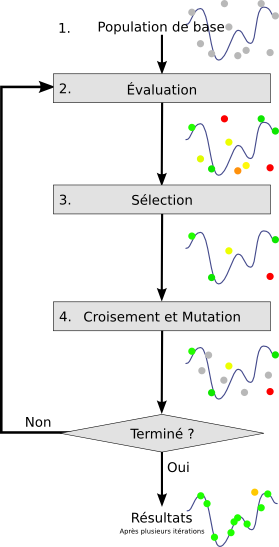
\includegraphics[width=.4\textwidth]{images/AG.png}
%%		\caption{Exemple d'algorithme génétique (source : wikipedia)}\label{fig:AG}
%%	\end{figure}
%%
%%
%%Si il est tout à fait logique que les algorithmes génétiques répondent parfaitement à la définition de l'évolution par sélection naturelle puisque ils ont été créés pour le faire, il est néanmoins intéressant de remarquer à quel point les roboticiens n'ont pas eu trop à les distordre pour s'en servir.
%%En effet, là où les informaticiens en algorithmique évolutionnaire classique ont souvent du ruser, détourner et ajouter de nombreux mécanismes \emph{ad-hoc} et sans équivalent biologique aux principes de base pour répondre aux problèmes qui leur étaient posés, les roboticiens n'ont bien souvent eux qu'à reprendre les premières formulations des algorithmes génétiques (cf. fig. \ref{fig:AG}), superposables quasi parfaitement avec la définition de Lewotin, pour obtenir de très bon résultats (pour une revue assez complète, voir \citet{nolfi00evolrobobiolintetechselfmach}, pour une revue plus récente : \citet{floreano10evolutionadaptivebehaviourrobotsbymeansdarwinianselection}).
%%
%%Tout comme en Informatique Évolutionnanrei les nuances et les ``écoles'' sont nombreuses. Il existent de nombreuses ``approches'' possibles.%citer la famille sisi
%%
%%
%%
